% =============================================================================
% HPT-QRC Concepts Guide — A Teacher's Explanation of Every Term in the Paper
% =============================================================================
\documentclass[11pt]{article}

\usepackage[utf8]{inputenc}
\usepackage{amsmath, amssymb, amsthm}
\DeclareMathOperator*{\argmin}{arg\,min}
\usepackage{booktabs}
\usepackage{graphicx}
\usepackage{float}
\usepackage[dvipsnames]{xcolor}
\usepackage{hyperref}
\usepackage{microtype}
\usepackage{geometry}
\usepackage{enumitem}
\usepackage{mdframed}
\usepackage{tcolorbox}
\usepackage{tikz}
\usepackage{array}
\usepackage{multirow}
\usepackage[T1]{fontenc}
\geometry{margin=1in}

\tcbuselibrary{skins, breakable}

\hypersetup{colorlinks=true, linkcolor=blue!50!black, citecolor=blue!50!black,
            urlcolor=blue!50!black}

% ---- Custom boxes ----
\tcbset{
  conceptbox/.style={
    enhanced, breakable,
    colback=blue!4!white,
    colframe=blue!50!black,
    fonttitle=\bfseries,
    attach boxed title to top left={yshift=-2mm, xshift=6mm},
    boxed title style={colback=blue!50!black, colframe=blue!50!black},
    top=4mm
  },
  mathbox/.style={
    enhanced, breakable,
    colback=orange!5!white,
    colframe=orange!70!black,
    fonttitle=\bfseries,
    attach boxed title to top left={yshift=-2mm, xshift=6mm},
    boxed title style={colback=orange!70!black},
    top=4mm
  },
  examplebox/.style={
    enhanced, breakable,
    colback=green!4!white,
    colframe=green!50!black,
    fonttitle=\bfseries,
    attach boxed title to top left={yshift=-2mm, xshift=6mm},
    boxed title style={colback=green!50!black},
    top=4mm
  },
  keybox/.style={
    enhanced,
    colback=red!4!white,
    colframe=red!60!black,
    fonttitle=\bfseries\large,
    top=2mm
  }
}

\newcommand{\concept}[2]{%
  \begin{tcolorbox}[conceptbox, title={#1}]
  #2
  \end{tcolorbox}
}
\newcommand{\mathblock}[2]{%
  \begin{tcolorbox}[mathbox, title={Math: #1}]
  #2
  \end{tcolorbox}
}
\newcommand{\example}[2]{%
  \begin{tcolorbox}[examplebox, title={Concrete Example: #1}]
  #2
  \end{tcolorbox}
}
\newcommand{\keypoint}[1]{%
  \begin{tcolorbox}[keybox]
  \textbf{Key Takeaway:} #1
  \end{tcolorbox}
}

\providecommand{\ket}[1]{\left| #1 \right\rangle}

\title{\textbf{Understanding the HPT-QRC Paper}\\[0.4em]
       \large A Complete Concept-by-Concept Teaching Guide\\[0.2em]
       \normalsize From Time-Series Forecasting to Quantum Photonics}

\author{Prepared for the HPT-QRC research team}
\date{May 2026}

\begin{document}

\maketitle
\tableofcontents
\clearpage

% =============================================================================
\section*{How to Use This Guide}
% =============================================================================
This guide is written like a textbook chapter. Every technical term used in the
paper ``Heterogeneous Photon-Number Ensembles in Linear-Optical Quantum Reservoir
Computing for Chaotic and Volatility Forecasting'' is explained from first
principles. You do not need a physics or statistics degree to follow along ---
just read in order. Each concept builds on the previous ones.

The guide is divided into five parts:
\begin{enumerate}
  \item \textbf{Time Series \& Statistics} --- AR, HAR, RV, MSE, QLIKE, Ridge
  \item \textbf{Machine Learning Foundations} --- ESN, RC, RFF, Optuna TPE, Walk-Forward
  \item \textbf{Statistical Inference} --- DM test, HAC variance, Andrews bandwidth, MCS
  \item \textbf{Quantum Photonics} --- Fock states, interferometers, SLOS, LexGrouping
  \item \textbf{Benchmarks \& Architecture} --- NARMA-10, Mackey-Glass, IPC, Virtual Depth
\end{enumerate}

\clearpage

% =============================================================================
\part{Time Series \& Statistics}
% =============================================================================

% -----------------------------------------------------------------------------
\section{AutoRegressive Models --- AR(1) and AR(3)}
% -----------------------------------------------------------------------------

\concept{What is an AutoRegressive Model?}{
Imagine you are trying to predict tomorrow's temperature. A simple strategy is:
``tomorrow's temperature is likely close to today's, plus some random variation.''
That is exactly what an AutoRegressive (AR) model does --- it predicts the next
value of a time series using a weighted sum of its own past values.

The ``order'' $p$ of an AR model (written AR($p$)) is simply \emph{how many
past values} you look back at. AR(1) looks 1 step back; AR(3) looks 3 steps
back.
}

\mathblock{AR($p$) Formula}{
\[
  y_t = c + \phi_1 y_{t-1} + \phi_2 y_{t-2} + \cdots + \phi_p y_{t-p}
        + \varepsilon_t, \qquad \varepsilon_t \sim \mathcal{N}(0, \sigma^2)
\]
\begin{itemize}
  \item $y_t$: the value we want to predict at time $t$
  \item $c$: a constant intercept (like an average level)
  \item $\phi_i$: the \emph{weight} given to the $i$-th past value
        (estimated from data by Ordinary Least Squares)
  \item $\varepsilon_t$: random noise --- unpredictable part
\end{itemize}

For \textbf{AR(1)}: $y_t = c + \phi_1 y_{t-1} + \varepsilon_t$

For \textbf{AR(3)}: $y_t = c + \phi_1 y_{t-1} + \phi_2 y_{t-2}
                              + \phi_3 y_{t-3} + \varepsilon_t$
}

\example{Volatility Persistence}{
Financial volatility is \emph{persistent} --- high-volatility days tend to be
followed by more high-volatility days. For S\&P 500 realized volatility,
$\hat\phi_1 \approx 0.85$ is typical:
\[
  \widehat{RV}_{t+1} \approx 0.003 + 0.85 \times RV_t
\]
So if today's RV is $0.02$, we forecast tomorrow's as
$0.003 + 0.85 \times 0.02 = 0.020$.
}

\keypoint{AR models are the \emph{floor} for forecasting. Any model worth
using should statistically beat them. In the paper they are the simplest
baselines in all three benchmarks.}

% -----------------------------------------------------------------------------
\section{HAR Model --- Heterogeneous AutoRegressive}
% -----------------------------------------------------------------------------

\concept{The Key Idea --- Multiple Horizons of Persistence}{
Financial markets are watched by many different types of participants. A
day trader looks at what happened in the last few hours. A hedge fund looks
at last week. A pension fund thinks in terms of months.

Corsi (2009) had a beautiful insight: \emph{realized volatility is the sum
of these overlapping, heterogeneous time horizons}. Rather than picking one
lag, why not include \emph{daily, weekly, and monthly} moving averages of
past volatility simultaneously? That is the HAR model.

Despite having only 4 parameters (intercept + three coefficients), HAR is
\textbf{notoriously hard to beat} --- deep learning models with millions
of parameters often cannot statistically outperform it on monthly RV data.
}

\mathblock{HAR Formula}{
\[
  RV_{t+1} = c + \beta_d \underbrace{RV_t}_{\text{daily}}
               + \beta_w \underbrace{\overline{RV}^{(5)}_t}_{\text{5-day avg}}
               + \beta_m \underbrace{\overline{RV}^{(22)}_t}_{\text{22-day avg}}
               + \varepsilon_{t+1}
\]

where:
\begin{align*}
  \overline{RV}^{(5)}_t  &= \tfrac{1}{5}(RV_t + RV_{t-1} + \cdots + RV_{t-4}) \\
  \overline{RV}^{(22)}_t &= \tfrac{1}{22}(RV_t + \cdots + RV_{t-21})
\end{align*}
The 4 parameters $c, \beta_d, \beta_w, \beta_m$ are estimated by OLS.
}

\example{Why HAR Wins on Monthly Data}{
S\&P 500 monthly realized volatility has a \emph{long memory} pattern ---
today's volatility is correlated with volatility from many months ago.
HAR approximates this long memory using a cascade of three short-memory
components: the daily component captures recent spikes; the weekly component
captures medium-term regimes; the monthly component captures structural
slow-moving volatility levels. Together they explain $\approx 70\%$ of
variance with only 4 parameters.
}

\paragraph{HARX (HAR with Exogenous Variables).}
HARX simply appends extra predictor variables $X_t$ to the HAR formula:
\[
  RV_{t+1} = c + \beta_d RV_t + \beta_w \overline{RV}^{(5)}_t
               + \beta_m \overline{RV}^{(22)}_t
               + \boldsymbol{\gamma}^\top \mathbf{X}_t + \varepsilon_{t+1}
\]
Common choices for $\mathbf{X}_t$: VIX (implied volatility), jump components,
bid-ask spreads. In the paper, Fama-French and macroeconomic factors are used
as exogenous inputs.

\keypoint{HAR is the primary classical rival for the S\&P 500 task. If
HPT-QRC (tuned) is statistically indistinguishable from HAR, that is a very
respectable result given HAR's strong track record.}

% -----------------------------------------------------------------------------
\section{Realized Volatility (RV)}
% -----------------------------------------------------------------------------

\concept{What is Realized Volatility?}{
``Volatility'' means how much asset prices fluctuate. Classical models
(like GARCH) treat volatility as a \emph{hidden} (latent) variable that
must be inferred from daily close-to-close returns. Realized Volatility is
different: it \emph{measures} volatility directly from high-frequency
(e.g., 5-minute) intraday data, treating it as if it were directly
observable.

This transforms a hard latent-variable estimation problem into a simple
regression problem: given today's observable RV, predict tomorrow's.
}

\mathblock{RV Formula}{
Given $M$ intraday log-returns $r_{t,j}$ over day $t$:
\[
  RV_t = \sum_{j=1}^{M} r_{t,j}^2,
  \qquad r_{t,j} = \log\!\left(\frac{P_{t,j}}{P_{t,j-1}}\right)
\]
For 5-minute returns over a 6.5-hour US trading day: $M = 78$.

As $M \to \infty$ (continuous sampling), by the theory of quadratic variation:
\[
  RV_t \xrightarrow{p} \int_0^1 \sigma^2_t \, dt + \sum_j J_j^2
\]
(integrated variance + squared jumps). So RV is a
\emph{model-free, consistent} estimator of total latent variance.
}

\keypoint{The S\&P~500 RV dataset covers 1950--2017 at monthly frequency.
Forecasting it well is the ``real-world relevance'' claim of the paper.}

% -----------------------------------------------------------------------------
\section{Ridge Regression}
% -----------------------------------------------------------------------------

\concept{Why Not Just Use Ordinary Least Squares (OLS)?}{
OLS finds the weights $\hat\beta$ that minimize the squared prediction error.
It works beautifully when you have many observations and few features. But when
the number of features is large (say, 270 quantum features from 3 reservoirs
$\times$ 3 virtual layers $\times$ 10 lex-out dimensions), OLS over-fits
badly: the coefficients become enormous and noisy, performing well on training
data but terribly on new data.

Ridge regression fixes this by adding a \emph{penalty} on the size of the
coefficients --- it shrinks them toward zero, sacrificing a tiny bit of
training accuracy for a huge gain in generalisation.
}

\mathblock{Ridge Objective and Solution}{
\textbf{Objective:}
\[
  \hat\beta_{\text{ridge}} = \argmin_\beta \,\|y - X\beta\|^2
                             + \alpha \|\beta\|^2
\]

\textbf{Closed-form solution:}
\[
  \hat\beta_{\text{ridge}} = (X^\top X + \alpha I)^{-1} X^\top y
\]

\begin{itemize}
  \item $\alpha > 0$: regularisation strength (tuned via Optuna)
  \item $\alpha I$: the identity times $\alpha$ added to $X^\top X$
        makes the matrix invertible even when features are correlated
  \item No iterative optimisation needed --- one matrix inversion
\end{itemize}

\textbf{Bias-variance tradeoff:}
\begin{itemize}
  \item Large $\alpha$: more shrinkage $\to$ higher bias, lower variance
  \item Small $\alpha$: less shrinkage $\to$ lower bias, higher variance
\end{itemize}
}

\example{Why Ridge is Perfect for Reservoir Computing}{
In HPT-QRC the reservoir (photonic circuit) is \emph{fixed} --- we never
train it. The only trainable component is the readout layer.
Ridge solves this in one shot:
\[
  W_{\text{out}} = (\Phi^\top \Phi + \alpha I)^{-1} \Phi^\top y
\]
where $\Phi \in \mathbb{R}^{T \times D}$ is the matrix of reservoir features.
For $D = 270$ features and $T = 800$ training samples, this is a tiny
$(270 \times 270)$ matrix inversion --- solved in milliseconds.
}

\keypoint{Ridge has no barren-plateau problem, no gradient descent, no
hyperparameter sensitivity beyond the single scalar $\alpha$. It is the
ideal readout for a fixed-reservoir architecture.}

% -----------------------------------------------------------------------------
\section{MSE and QLIKE Loss Functions}
% -----------------------------------------------------------------------------

\concept{Two Ways to Measure Forecast Error}{
A loss function quantifies ``how wrong'' a forecast is. Different loss
functions reward different properties.
}

\mathblock{MSE --- Mean Squared Error}{
\[
  \mathcal{L}_{\text{MSE}} = \frac{1}{T}\sum_{t=1}^{T}(\hat{y}_t - y_t)^2
\]
\begin{itemize}
  \item Symmetric: overestimating and underestimating by the same amount
        are penalised equally
  \item Scale-dependent: a 0.001 error is treated the same whether
        $y = 0.001$ or $y = 1000$
  \item Sensitive to outliers (squaring magnifies large errors)
\end{itemize}
}

\mathblock{QLIKE --- Quasi-Likelihood Loss}{
\[
  \mathcal{L}_{\text{QLIKE}}(\hat\sigma^2, \sigma^2)
  = \frac{\sigma^2}{\hat\sigma^2} - \log\!\frac{\sigma^2}{\hat\sigma^2} - 1
\]
\begin{itemize}
  \item Always $\geq 0$; equals 0 iff $\hat\sigma^2 = \sigma^2$
  \item \textbf{Scale-invariant}: penalises relative errors,
        not absolute ones
  \item \textbf{Asymmetric}: strongly penalises \emph{underestimating}
        volatility (dangerous in risk management: you think it's calm
        when it isn't)
  \item \textbf{Patton (2011)}: QLIKE is \emph{robust to noisy proxies} ---
        using a noisy RV estimate instead of true variance still correctly
        ranks forecasting models
\end{itemize}
}

\example{Why QLIKE $>$ MSE for Volatility}{
Suppose two forecasters predict next-month S\&P~500 RV:
\begin{center}
\begin{tabular}{lcccc}
\toprule
& True $\sigma^2$ & Forecast $\hat\sigma^2$ & MSE & QLIKE \\
\midrule
Forecaster A & 0.010 & 0.012 & $4\!\times\!10^{-6}$ & 0.003 \\
Forecaster B & 0.010 & 0.002 & $64\!\times\!10^{-6}$ & 1.609 \\
\midrule
Forecaster A & 0.100 & 0.102 & $4\!\times\!10^{-6}$ & 0.000 \\
Forecaster B & 0.100 & 0.020 & $6400\!\times\!10^{-6}$ & 1.609 \\
\bottomrule
\end{tabular}
\end{center}
MSE treats Forecaster A the same at low and high volatility.
QLIKE recognises that underestimating by a factor of 5 (Forecaster B)
is catastrophic from a risk-management perspective.
}

\keypoint{In the paper, QLIKE is the \emph{primary} metric for the S\&P~500
task. All DM tests are run on both MSE and QLIKE. QLIKE is even reported
on the synthetic benchmarks (NARMA-10, Mackey-Glass) for uniform comparability
across datasets.}

% =============================================================================
\clearpage
\part{Machine Learning Foundations}
% =============================================================================

% -----------------------------------------------------------------------------
\section{Reservoir Computing and Echo State Networks (ESN)}
% -----------------------------------------------------------------------------

\concept{Reservoir Computing --- The Big Idea}{
Training a Recurrent Neural Network (RNN) is hard: gradients either
\emph{explode} or \emph{vanish} as they flow through time (the
vanishing-gradient problem). Reservoir Computing sidesteps this entirely
by \textbf{never training the recurrent part at all}.

The idea:
\begin{enumerate}
  \item Take a complex dynamical system (the ``reservoir'') with random,
        \emph{fixed} connections.
  \item Drive it with your input time series.
  \item The reservoir maps the history of inputs into a rich
        high-dimensional state space.
  \item Train \emph{only} a simple linear readout from reservoir states
        to outputs.
\end{enumerate}
This is like having a pre-built pattern recogniser (the reservoir) and
only learning how to \emph{read} its outputs.
}

\mathblock{Echo State Network (ESN) Equations}{
\textbf{Reservoir state update:}
\[
  \mathbf{x}_t = (1-\alpha)\mathbf{x}_{t-1}
                + \alpha \cdot \tanh\!\bigl(W_{\text{in}}\, u_t
                                           + W_{\text{res}}\, \mathbf{x}_{t-1}\bigr)
\]

\textbf{Readout (only trained part):}
\[
  \hat y_t = W_{\text{out}}\, \mathbf{x}_t
\]

\begin{itemize}
  \item $\mathbf{x}_t \in \mathbb{R}^N$: reservoir state ($N \approx 200$--$1000$)
  \item $W_{\text{res}} \in \mathbb{R}^{N\times N}$: random sparse fixed matrix,
        spectral radius $\rho < 1$
  \item $W_{\text{in}}$: random fixed input matrix
  \item $\alpha \in (0,1]$: leaking rate --- controls speed of state update
  \item $W_{\text{out}}$: \textbf{only trained weights}, via Ridge regression
\end{itemize}

\textbf{Echo State Property (ESP):} With $\rho(W_{\text{res}}) < 1$, the
reservoir ``forgets'' its initial state exponentially fast. The current
state $\mathbf{x}_t$ depends only on the recent input history, not on
arbitrary initial conditions.
}

\example{Why ESN is the Main Baseline in the Paper}{
ESN and HPT-QRC share the same structure:
\begin{center}
\begin{tabular}{lll}
\toprule
& ESN & HPT-QRC \\
\midrule
Reservoir type & Random RNN (classical) & Photonic interferometer \\
Reservoir training & None (fixed) & None (fixed) \\
Readout training & Ridge regression & Ridge regression \\
Memory source & Recurrent connections & Sliding window + Fock states \\
\bottomrule
\end{tabular}
\end{center}
Comparing them is ``apples-to-apples'' for the reservoir computing paradigm.
}

\keypoint{ESN is swept over sizes $\{50, 100, 200, 500, 1000\}$ with Optuna
tuning of leak rate, spectral radius, and ridge $\alpha$. It is the most
competitive classical reservoir baseline.}

% -----------------------------------------------------------------------------
\section{Random Fourier Features (RFF)}
% -----------------------------------------------------------------------------

\concept{Kernel Methods Without the $O(T^2)$ Cost}{
Kernel methods (like SVMs) find nonlinear patterns by implicitly operating
in a high-dimensional feature space via a kernel function
$k(\mathbf{x}, \mathbf{y})$. The catch: computing $k$ for all pairs of
$T$ training points costs $O(T^2)$ --- too slow for large datasets.

Rahimi \& Recht (NeurIPS 2007) had an elegant idea: instead of computing
the kernel implicitly, \emph{approximate it explicitly} using random
projections. Their Random Fourier Features map inputs into a
$D$-dimensional feature space where the dot product $\approx$ the kernel.
Then just run linear regression on these features.
}

\mathblock{RFF Construction (RBF Kernel)}{
For the Radial Basis Function (RBF) kernel $k(x,y) = e^{-\|x-y\|^2 / 2\sigma^2}$:

1.\ Sample $D$ random frequencies: $\boldsymbol\omega_j \sim \mathcal{N}(0,
   \sigma^{-2} I)$, and offsets $b_j \sim \mathcal{U}[0, 2\pi]$

2.\ Feature map:
\[
  \phi(\mathbf{x}) = \sqrt{\tfrac{2}{D}}
  \bigl[\cos(\boldsymbol\omega_1^\top \mathbf{x} + b_1),\;
        \ldots,\;
        \cos(\boldsymbol\omega_D^\top \mathbf{x} + b_D)\bigr]
\]

3.\ By Bochner's theorem: $k(\mathbf{x}, \mathbf{y})
    \approx \phi(\mathbf{x})^\top \phi(\mathbf{y})$

Then fit Ridge regression: $\hat y = \hat\beta^\top \phi(\mathbf{x})$.
}

\keypoint{In the paper, RFF+Ridge is the \emph{matched-dimension kernel
baseline} --- tuned to the same feature dimension as HPT-QRC via Optuna.
It tests whether HPT-QRC's quantum Fock features are better than a
carefully tuned classical kernel method of the same size.}

% -----------------------------------------------------------------------------
\section{Optuna and the TPE Algorithm}
% -----------------------------------------------------------------------------

\concept{Hyperparameter Optimisation --- Why it Matters}{
Every machine learning model has ``dials'' that must be set before training:
learning rate, number of layers, regularisation strength, window size, etc.
These are called \emph{hyperparameters}. The right settings can be the
difference between a model that works and one that doesn't.

\textbf{Grid search}: try every combination --- $O(k^d)$ evaluations for
$d$ hyperparameters, each with $k$ values. Exponentially expensive.

\textbf{Random search}: try random combinations --- better, but ignores
what was learned from previous trials.

\textbf{Bayesian optimisation} (Optuna's approach): model which
hyperparameter regions are promising and \emph{focus} evaluations there.
}

\mathblock{TPE --- Tree-structured Parzen Estimator}{
At each step, Optuna splits all previous trials into:
\begin{itemize}
  \item $\ell(\lambda)$: density of ``good'' configs (top $\gamma = 25\%$ by loss)
  \item $g(\lambda)$: density of ``bad'' configs (bottom $75\%$)
\end{itemize}
Both are estimated as \emph{Parzen windows} (mixture of Gaussians).

The next hyperparameter to try maximises:
\[
  \text{EI}(\lambda) \propto \frac{\ell(\lambda)}{g(\lambda)}
  \quad \text{(Expected Improvement)}
\]

\textbf{Why TPE is practical:}
\begin{itemize}
  \item Handles continuous, integer, and categorical hyperparameters
  \item Handles conditional structure (e.g., ``if model is LSTM, tune
        \texttt{n\_layers}'')
  \item No matrix inversions --- fast and scalable
  \item Default sampler in Optuna (the most popular HPO library)
\end{itemize}
}

\example{HPT-QRC Hyperparameter Search Space}{
Optuna tunes 5 hyperparameters for HPT-QRC:
\begin{center}
\begin{tabular}{lll}
\toprule
Hyperparameter & Range & Best (Mackey-Glass) \\
\midrule
\texttt{photon\_list} & $\{[2],[3],[4],[2,3],[2,4],[3,4],[2,3,4]\}$ & $[2,4]$ \\
\texttt{window} & $1$--$20$ & $5$ \\
\texttt{n\_virtual\_nodes} & $1$--$5$ & $3$ \\
\texttt{lex\_out} & $4$--$20$ & $14$ \\
\texttt{ridge\_alpha} & $10^{-8}$--$10^{-1}$ (log scale) & $10^{-6}$ \\
\bottomrule
\end{tabular}
\end{center}
20 Optuna trials (fewer than 30 for classical baselines, since each
HPT-QRC fit is slower).
}

\keypoint{Because HPT-QRC uses \emph{fewer} trials (20 vs 30), any
performance advantage is \emph{conservative} --- the quantum model is
actually at a slight search disadvantage.}

% -----------------------------------------------------------------------------
\section{Walk-Forward Validation}
% -----------------------------------------------------------------------------

\concept{Why Standard Cross-Validation is Dangerous for Time Series}{
Standard $k$-fold cross-validation randomly shuffles your data and trains
on some folds, tests on others. For i.i.d.\ data (e.g., image classification)
this is fine. For time series it is \textbf{catastrophic}: if you train on
data from 2020 and test on data from 2015, you are effectively ``looking
into the past from the future'' --- the model sees future information
during training. This is called \emph{look-ahead bias} and produces
overly optimistic results.

Walk-forward validation fixes this by always respecting the arrow of time:
\textbf{train on the past, test on the future}.
}

\mathblock{Walk-Forward Protocol in the Paper}{
For S\&P~500 RV (1950--2017, 68 years of monthly data):
\begin{itemize}
  \item Train window: 20 years
  \item Validation window: 2 years (for hyperparameter selection)
  \item Test window: 2 years
  \item Slide: 2 years forward after each fold
  \item Total folds: 8 (covering 1970--2017)
\end{itemize}

\begin{center}
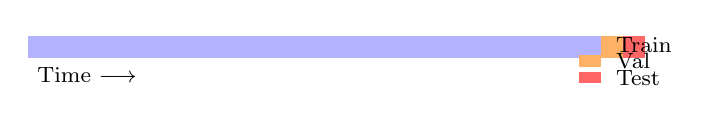
\begin{tikzpicture}[scale=0.7]
  \foreach \i in {0,...,7} {
    \fill[blue!30] (\i*1.2, 0) rectangle (\i*1.2 + 2.0, 0.4);
    \fill[orange!60] (\i*1.2 + 2.0, 0) rectangle (\i*1.2 + 2.4, 0.4);
    \fill[red!60] (\i*1.2 + 2.4, 0) rectangle (\i*1.2 + 2.8, 0.4);
  }
  \node[anchor=west] at (0, -0.3) {\footnotesize Time $\longrightarrow$};
  \fill[blue!30] (10, 0.15) rectangle (10.4, 0.35);
  \node[anchor=west, font=\footnotesize] at (10.5, 0.25) {Train};
  \fill[orange!60] (10, -0.15) rectangle (10.4, 0.05);
  \node[anchor=west, font=\footnotesize] at (10.5, -0.05) {Val};
  \fill[red!60] (10, -0.45) rectangle (10.4, -0.25);
  \node[anchor=west, font=\footnotesize] at (10.5, -0.35) {Test};
\end{tikzpicture}
\end{center}

Results are reported as \emph{median} and IQR across the 8 test folds.
}

\keypoint{Walk-forward is harder than a fixed 80/20 split.
HPT-QRC (default config) trails HAR in walk-forward median MSE. The
paper is transparent about this --- the tuned walk-forward result
is deferred to the journal version.}

% =============================================================================
\clearpage
\part{Statistical Inference}
% =============================================================================

% -----------------------------------------------------------------------------
\section{The Diebold-Mariano (DM) Test}
% -----------------------------------------------------------------------------

\concept{Are Two Forecasters Really Different, or Just Lucky?}{
Suppose Model A has lower MSE than Model B on a test set of 100 months.
Is A genuinely better, or did it just happen to be luckier on these particular
100 months? The Diebold-Mariano (DM) test answers this question rigorously
using hypothesis testing.

Think of it as the forecasting equivalent of a two-sample t-test.
}

\mathblock{DM Test Step-by-Step}{
\textbf{Step 1.} Compute loss differential at each time point:
\[
  d_t = L(\hat y^A_t, y_t) - L(\hat y^B_t, y_t)
\]
e.g., $d_t = (\hat y^A_t - y_t)^2 - (\hat y^B_t - y_t)^2$ for MSE.

\textbf{Step 2.} Null hypothesis:
\[
  H_0: \mathbb{E}[d_t] = 0 \quad \text{(equal expected accuracy)}
\]

\textbf{Step 3.} Test statistic:
\[
  DM = \frac{\bar d}{\sqrt{\widehat{\mathrm{Var}}(\bar d)}}
     \;\xrightarrow{d}\; \mathcal{N}(0,1)
\]
where $\bar d = \frac{1}{T}\sum_t d_t$ and $\widehat{\mathrm{Var}}(\bar d)$
is a HAC variance estimate (see Section~\ref{sec:hac}).

\textbf{Step 4.} For a two-sided test at 5\% level:
reject $H_0$ if $|DM| > 1.96$.

\textbf{Interpretation:}
\begin{itemize}
  \item $DM > 0$ (and significant): Model B is better (A has higher loss)
  \item $DM < 0$ (and significant): Model A is better (B has higher loss)
  \item $|DM| < 1.96$: cannot tell them apart at 5\% level
\end{itemize}
}

\example{Reading Table~5 in the Paper}{
For HPT-QRC (tuned) vs.\ HAR on S\&P~500 RV:
\begin{center}
\begin{tabular}{lcc}
\toprule
Metric & DM stat & $p$-value \\
\midrule
MSE & 1.979 & 0.048 \\
QLIKE & 1.732 & 0.083 \\
\bottomrule
\end{tabular}
\end{center}
$DM = 1.979 > 0$ means HAR has lower MSE than HPT-QRC.
$p = 0.048 < 0.05$: statistically significant at 5\%.

\textbf{Translation:} ``HAR beats HPT-QRC on MSE at the 5\% significance
level. However, on QLIKE ($p = 0.083 > 0.05$), we cannot distinguish
them.'' This is consistent with HPT-QRC being ``in the same statistical
class'' as HAR --- it doesn't clearly beat HAR, but also isn't clearly
worse on the volatility-appropriate loss.
}

\keypoint{The DM test is the core of the paper's statistical claims.
Without it, saying ``Model A has lower error than Model B'' is just
descriptive --- it could be noise. The DM test says whether the
difference is real.}

% -----------------------------------------------------------------------------
\section{Newey-West HAC Variance}\label{sec:hac}
% -----------------------------------------------------------------------------

\concept{Why Regular Standard Errors are Wrong for Forecast Errors}{
In a standard regression, error terms are assumed to be independent
(i.i.d.). But forecast errors are \emph{not} independent: if you
underestimate volatility today, you'll likely underestimate it tomorrow
too (serial correlation). Also, errors vary in size over time
(heteroskedasticity --- think calm vs.\ volatile market periods).

Using standard error formulas under these violations \emph{underestimates}
the true variance of $\bar d$, making the DM statistic look larger
(more significant) than it really is --- you'd get spurious p-values.

HAC stands for \textbf{H}eteroskedasticity and \textbf{A}utocorrelation
\textbf{C}onsistent. The Newey-West estimator corrects for both problems.
}

\mathblock{Newey-West (1987) HAC Estimator}{
\[
  \hat V_{\text{HAC}} = \hat\Gamma_0
    + \sum_{j=1}^{m} w_j \bigl(\hat\Gamma_j + \hat\Gamma_j^\top\bigr)
\]

where the $j$-th autocovariance is:
\[
  \hat\Gamma_j = \frac{1}{T}\sum_{t=j+1}^{T} d_t \cdot d_{t-j}
\]

and Bartlett kernel weights are:
\[
  w_j = 1 - \frac{j}{m+1}, \quad j = 1, \ldots, m
\]

The bandwidth $m$ controls how many lags of autocorrelation to account for.
}

\mathblock{Andrews (1991) Automatic Bandwidth}{
How large should $m$ be? Too small: miss important autocorrelations.
Too large: add noisy lag estimates. Andrews (1991) derived the
asymptotically optimal data-driven choice:
\[
  m^* = \left\lfloor 4 \left(\frac{T}{100}\right)^{2/9} \right\rfloor
\]

For $T = 135$ monthly observations: $m^* = \lfloor 4 \times (1.35)^{2/9}
\rfloor = \lfloor 4 \times 1.068 \rfloor = 4$.

This formula comes from minimising the asymptotic mean squared error of
the HAC estimator under the Bartlett kernel.
}

\keypoint{Every DM $p$-value in the paper uses HAC standard errors with
the Andrews automatic bandwidth. This is the \emph{econometrically
correct} way to run DM tests --- most ML papers skip this step and
get over-confident p-values.}

% -----------------------------------------------------------------------------
\section{Hansen Model Confidence Set (MCS)}
% -----------------------------------------------------------------------------

\concept{The Multiple Comparisons Problem}{
If you compare 10 models pairwise with 5\% tests, you'd run $\binom{10}{2}=45$
tests. Even if all models are identical, you expect $45 \times 0.05 \approx 2$
false positives. This is the \emph{multiple comparisons problem} --- you
can't just run many DM tests and collect ``significant'' results.

Hansen's Model Confidence Set (2011) solves this by producing a
\emph{set of models} that cannot be distinguished from the best model at a
given confidence level --- a ``confidence interval for the identity of
the best model.''
}

\mathblock{MCS Algorithm}{
\textbf{Input:} Set of models $\mathcal{M}_0$, confidence level $\alpha = 0.10$.

\textbf{Algorithm:}
\begin{enumerate}
  \item Test $H_0^{\mathcal{M}}$: all models in $\mathcal{M}$ have equal
        expected loss (using stationary bootstrap for $p$-values)
  \item If $H_0$ \emph{not rejected}: stop. Current $\mathcal{M}$ is the MCS.
  \item If $H_0$ \emph{rejected}: remove the worst model
        (highest average loss differential vs.\ others) from $\mathcal{M}$,
        go to step 1.
\end{enumerate}

\textbf{Output:} $\hat{\mathcal{M}}^*_{1-\alpha}$ --- the 90\% MCS survivor set.

\textbf{Interpretation:} Models in the MCS are statistically indistinguishable
from the best model. Being in the MCS is the forecasting analogue of
``not significantly worse than the winner.''
}

\example{MCS Results in the Paper}{
For S\&P 500 RV (fixed split), the MCS retains \emph{all} 14 models with
$p = 0.39$ --- with only $T \approx 135$ test months, the data does not
have enough power to separate any model from the best. This is the
standard finding in the RV forecasting literature: HAR and its competitors
are hard to distinguish at monthly frequency with real data.

For walk-forward (8 folds, $T = 192$ test points combined): all 8 models
in the MCS (MSE: $p = 0.125$, QLIKE: $p = 0.312$). Same conclusion.
}

\paragraph{Stationary Bootstrap.}
The MCS uses bootstrap to generate critical values. The
\emph{stationary bootstrap} (Politis \& Romano 1994) resamples blocks of
data with \emph{geometrically distributed random lengths} (mean block
length $= 20$ in the paper), preserving the autocorrelation structure
of the loss differential series. The paper uses $B = 2000$ bootstrap
resamples.

\keypoint{The MCS + DM combination is the gold standard for forecast
comparison in econometrics. The paper uses it correctly --- this is
what makes it publishable in econometrics venues.}

% =============================================================================
\clearpage
\part{Quantum Photonics}
% =============================================================================

% -----------------------------------------------------------------------------
\section{Quantum States and Fock Space}
% -----------------------------------------------------------------------------

\concept{Particles That Are All Identical --- Bosons}{
In everyday life, objects are distinguishable: ``the red ball'' vs.\ ``the blue ball.'' Quantum particles are different. \emph{Bosons} (like photons, the particles of light) are \textbf{fundamentally indistinguishable} --- there is no ``photon number 1'' vs.\ ``photon number 2.'' The only meaningful question is: ``how many photons are in each location (mode)?''

An optical ``mode'' is a specific spatial/temporal/polarisation channel that a photon can occupy. Think of modes as slots in a box.
}

\mathblock{Fock States}{
A \emph{Fock state} specifies the occupation number of each mode:
\[
  \ket{n_1, n_2, \ldots, n_m}
\]
$n_i$ = number of photons in mode $i$.

\textbf{Example:} $\ket{1, 0, 2, 0}$ means: mode 1 has 1 photon, mode 3 has 2 photons, modes 2 and 4 are empty. Total: 3 photons in 4 modes.

\textbf{Counting Fock states} with exactly $n$ photons in $m$ modes:
\[
  \text{Full Fock space}: \binom{n+m-1}{n} \quad \text{(stars-and-bars)}
\]
\[
  \text{Unbunched (max 1 per mode)}: \binom{m}{n}
\]

\textbf{Concrete sizes:}
\begin{center}
\begin{tabular}{ccccc}
\toprule
$n$ & $m$ & Full & Unbunched & HPT-QRC \\
\midrule
2 & 6 & 21 & 15 & $\binom{6}{2}=15$ \\
3 & 6 & 56 & 20 & $\binom{6}{3}=20$ \\
4 & 6 & 126 & 15 & $\binom{6}{4}=15$ \\
\bottomrule
\end{tabular}
\end{center}
}

\keypoint{Fock states are the ``vocabulary'' of photonic computing.
The HPT-QRC paper extracts the \emph{probability} of each Fock state
at the output of the interferometer and uses these probabilities as
features for regression.}

% -----------------------------------------------------------------------------
\section{Linear Optical Interferometers and Phase Encoding}
% -----------------------------------------------------------------------------

\concept{What is a Photonic Interferometer?}{
An optical interferometer is a network of beam splitters and phase shifters
that redirects and mixes light beams. Mathematically it implements a
\emph{unitary transformation} $U$ on the photon mode operators.

Think of it as a ``photon mixer'': photons entering from the left emerge
at the right with transformed probabilities, governed by interference.
}

\mathblock{Building Blocks}{
\textbf{Beam Splitter (BS):} Mixes two modes with reflectivity $\theta$:
\[
  \begin{pmatrix} b_1 \\ b_2 \end{pmatrix}
  = \begin{pmatrix} \cos\theta & i\sin\theta \\ i\sin\theta & \cos\theta
    \end{pmatrix}
  \begin{pmatrix} a_1 \\ a_2 \end{pmatrix}
\]
A 50:50 BS ($\theta = \pi/4$) sends half the photons to each output.

\textbf{Phase Shifter (PS):} Multiplies a mode by a phase:
\[
  b = e^{i\phi} a
\]
This is the \textbf{encoding mechanism} in HPT-QRC: the time-series
input $x_t \in [0,1]$ is encoded as $\phi = 2\pi x_t$.

\textbf{Mach-Zehnder Interferometer (MZI):}
Two 50:50 beam splitters with a phase shifter between them --- a
tunable beam splitter with continuously adjustable splitting ratio.
Cascading MZIs can implement \emph{any} unitary transformation.
}

\concept{How Input Is Encoded into the Circuit}{
\textbf{Step 1.} Take the time-series window
$\mathbf{x}_t = [y_{t-W+1}, \ldots, y_t]$ (e.g., 10 past values).

\textbf{Step 2.} Winsorise and min-max scale to $[0,1]$.

\textbf{Step 3.} Each value controls one input phase shifter:
$\phi_k = 2\pi x_{t-W+k}$.

\textbf{Step 4.} The Fock input state $\ket{1^n 0^{m-n}}$
($n$ photons in the first $n$ modes, rest empty) enters the phase-encoded circuit.

\textbf{Step 5.} The circuit's fixed random beam splitter network
(the ``reservoir'') mixes these phase-encoded modes through
quantum interference.

\textbf{Step 6.} Measure the output Fock probabilities --- these are the features.
}

\keypoint{The fixed random interferometer parameters are the ``reservoir''
--- they are never trained. Only the input phase encoding changes with
each time step. This is analogous to how ESN reservoir weights are random
and fixed, but input weights map the current input to the reservoir.}

% -----------------------------------------------------------------------------
\section{The Permanent of a Matrix and Boson Sampling}
% -----------------------------------------------------------------------------

\concept{Why Photon Counting is Hard to Simulate Classically}{
When $n$ indistinguishable photons pass through an $m$-mode interferometer,
the output probabilities involve a mathematical quantity called the
\emph{permanent} of a matrix. Computing the permanent is among the
hardest problems in mathematics.
}

\mathblock{Permanent vs.\ Determinant}{
For an $n \times n$ matrix $A$:

\[
  \det(A)  = \sum_{\sigma \in S_n} \underbrace{\text{sgn}(\sigma)}_{\pm 1}
             \prod_{i=1}^n a_{i,\sigma(i)}
  \quad \text{(computable in } O(n^3))
\]
\[
  \text{Perm}(A) = \sum_{\sigma \in S_n}
                  \prod_{i=1}^n a_{i,\sigma(i)}
  \quad \text{(no sign! computable in } O(2^n n))
\]

The \emph{only} difference is the absence of the sign $\text{sgn}(\sigma)$.
Yet this makes the permanent \textbf{\#P-hard} to compute (Valiant 1979) ---
believed to be harder than NP.

\textbf{Fock state transition probability:}
\[
  P(|S\rangle \to |T\rangle) = \frac{|\text{Perm}(U_{ST})|^2}{\prod_i s_i!\,\prod_j t_j!}
\]
where $U_{ST}$ is the submatrix of the interferometer unitary $U$ formed
by selecting columns per input state $S$ and rows per output state $T$.
}

\concept{Boson Sampling (Aaronson-Arkhipov 2011)}{
\textbf{Task:} Sample from the output Fock distribution of a random $m$-mode
interferometer with $n \ll m$ photons.

\textbf{Computational claim:} No polynomial-time classical algorithm exists
for this (unless the polynomial hierarchy collapses).

\textbf{Why it matters for HPT-QRC:}
The features extracted by HPT-QRC come from this distribution.
In principle, they represent a classically hard-to-reproduce probability
distribution. \emph{Note:} The paper explicitly does \textbf{NOT} claim
quantum advantage for regression --- only that Fock-space features are
expressive and useful.
}

% -----------------------------------------------------------------------------
\section{Perceval, SLOS, and MerLin}
% -----------------------------------------------------------------------------

\concept{Perceval --- The Photonic Simulation Engine}{
Perceval is Quandela's open-source Python library for simulating photonic
quantum circuits. Think of it as PyTorch for photonic computing.

\textbf{Key idea:} You describe a circuit (beam splitters, phase shifters,
photon sources, detectors). Perceval simulates what happens to the photons
and returns output probabilities.
}

\mathblock{SLOS Backend --- Scalable Linear Optical Simulator}{
The default exact simulation backend. For $n$ photons in $m$ modes:

\textbf{Algorithm:}
\begin{enumerate}
  \item Start with input Fock state $\ket{n_1,\ldots,n_m}$
  \item Propagate amplitude column-by-column through the circuit,
        contracting the bosonic Hilbert space at each step
  \item The result: a full output probability distribution over
        all valid Fock states
\end{enumerate}

\textbf{Complexity:} $O\!\left(\binom{n+m-1}{n} \cdot m\right)$
--- polynomial in $m$ for fixed $n$, but exponential in $n$.

\textbf{Why SLOS is exact:} Unlike approximations (neural-network surrogate
models, sampling methods), SLOS computes exact permanents, giving
exact Fock probabilities. This is crucial for HPT-QRC --- we need
deterministic, noise-free features from the simulation.
}

\concept{ComputationSpace.UNBUNCHED --- At Most One Photon Per Mode}{
When we restrict to the \textbf{unbunched} subspace, we only consider
Fock states where every mode has 0 or 1 photon ($n_i \in \{0,1\}$).

\textbf{Why unbunched:}
\begin{itemize}
  \item Smaller feature space: $\binom{m}{n}$ instead of $\binom{n+m-1}{n}$
  \item Easier to implement experimentally: coincidence detection
        (one photon per detector at a time) is standard hardware
  \item On real hardware (Ascella), bunched events are identified by
        photon-number-resolving detectors and \emph{discarded} via
        post-selection, recovering the unbunched distribution
\end{itemize}
}

\concept{MerLin --- Differentiable Photonic ML on Perceval}{
MerLin wraps Perceval circuits into PyTorch \texttt{nn.Module} objects,
enabling integration with standard deep learning pipelines.

In HPT-QRC, the key MerLin component is \texttt{QuantumLayer}:
a fixed photonic circuit whose forward pass returns Fock output
probabilities. No gradients flow through the circuit (reservoir
is frozen) --- only the Ridge readout is trained.
}

% -----------------------------------------------------------------------------
\section{LexGrouping --- Compressing Fock Probabilities}
% -----------------------------------------------------------------------------

\concept{The Dimensionality Problem}{
After SLOS simulation in the unbunched subspace, we have
$\binom{m}{n}$ output probabilities. For the heterogeneous ensemble
$[2,3,4]$ photons with $m = 6$ modes:
\[
  \binom{6}{2} + \binom{6}{3} + \binom{6}{4} = 15 + 20 + 15 = 50
  \text{ features per virtual layer}
\]
With 3 virtual layers: $150$ features. But we want to control this
flexibly. LexGrouping does this compression.
}

\mathblock{LexGrouping Algorithm}{
Given $K = \binom{m}{n}$ Fock probabilities $p_1, \ldots, p_K$
(indexed in lexicographic order of Fock states):

\textbf{Step 1.} Pad to $K' = \lceil K/D \rceil \cdot D$ by appending zeros.

\textbf{Step 2.} Divide into $D$ contiguous groups of $\lceil K/D\rceil$ each.

\textbf{Step 3.} Sum within each group:
\[
  [\text{LexGroup}(\mathbf{p})]_d
  = \sum_{k=(d-1)\lceil K/D\rceil}^{d\lceil K/D\rceil-1} p_k,
  \quad d = 1, \ldots, D
\]

\textbf{Result:} A $D$-dimensional vector. Total probability is preserved
($\sum_d [\text{LexGroup}]_d = \sum_k p_k$). $D$ is the tunable
hyperparameter \texttt{lex\_out}.
}

\example{LexGrouping with 6 Fock States into 3 Groups}{
Unbunched states for $n=2$, $m=4$:
$\ket{1100}, \ket{1010}, \ket{1001}, \ket{0110}, \ket{0101}, \ket{0011}$
with probabilities $[0.3, 0.1, 0.05, 0.2, 0.15, 0.2]$.

LexGroup into $D=3$ groups (2 states per group):
\begin{align*}
  g_1 &= 0.3 + 0.1 = 0.40 \\
  g_2 &= 0.05 + 0.2 = 0.25 \\
  g_3 &= 0.15 + 0.2 = 0.35
\end{align*}
Output: $[0.40,\; 0.25,\; 0.35]$ --- sums to 1.0. $\checkmark$
}

\keypoint{LexGrouping is a parameter-free, deterministic compression that
preserves total probability. It is not a learned layer --- no training
required. The tunable parameter is simply $D$ (\texttt{lex\_out}), which
controls feature dimension.}

% =============================================================================
\clearpage
\part{Benchmarks and Architecture}
% =============================================================================

% -----------------------------------------------------------------------------
\section{NARMA-10 Benchmark}
% -----------------------------------------------------------------------------

\concept{A Nonlinear Memory Challenge}{
NARMA stands for Nonlinear AutoRegressive Moving Average. NARMA-10 is a
synthetic time series that requires a model to:
\begin{itemize}
  \item Integrate information from the last \emph{10} time steps (memory)
  \item Combine past outputs and past inputs \emph{nonlinearly}
  \item No purely linear method can solve it optimally
\end{itemize}
It is the most widely used synthetic benchmark in reservoir computing literature.
}

\mathblock{Exact NARMA-10 Formula}{
\[
  y_{t+1} = 0.3\, y_t + 0.05\, y_t \sum_{i=0}^{9} y_{t-i}
           + 1.5\, u_{t-9}\, u_t + 0.1
\]
where $u_t \sim \mathcal{U}[0, 0.5]$ is the driving input.

\textbf{Breakdown:}
\begin{itemize}
  \item $0.3\, y_t$: linear AR(1) component
  \item $0.05\, y_t \sum_{i=0}^{9} y_{t-i}$: nonlinear term coupling
        current output to sum of 10 past outputs
  \item $1.5\, u_{t-9}\, u_t$: input product term --- requires memory
        of at least 9 steps
\end{itemize}

\textbf{Metric:} Normalised MSE (NMSE) = $\text{MSE}/\text{Var}(y)$.
NMSE = 1.0 means the model is no better than predicting the mean.
}

\example{Why NARMA-10 Favours HPT-QRC}{
The IPC analysis in the paper shows that HPT-QRC achieves $\approx 1.3\times$
more degree-3 nonlinear capacity than ESN at matched feature dimension.
The nonlinear terms in NARMA-10 (especially the product $u_{t-9} \cdot u_t$)
require exactly this cubic-order processing. This is why HPT-QRC-X achieves
$3.98 \times 10^{-4}$ MSE vs.\ RFF+Ridge-X's $4.36 \times 10^{-4}$.
}

% -----------------------------------------------------------------------------
\section{Mackey-Glass Benchmark}
% -----------------------------------------------------------------------------

\concept{A Classic Chaotic System}{
The Mackey-Glass equation was originally proposed in 1977 as a model of
blood cell regulation with time-delayed feedback. For the right parameter
setting, it produces \emph{chaotic} dynamics: the system is entirely
deterministic but its long-run behaviour is unpredictable (sensitive to
initial conditions).

It is the standard ``hard'' time-series benchmark in reservoir computing.
}

\mathblock{Mackey-Glass Equation}{
\[
  \frac{dx}{dt} = \frac{\beta\, x(t - \tau)}{1 + x(t-\tau)^n} - \gamma\, x(t)
\]
Standard parameters: $\beta = 0.2$, $\gamma = 0.1$, $n = 10$.

\textbf{Chaos parameter $\tau$:}
\begin{itemize}
  \item $\tau < 17$: periodic oscillations (not chaotic)
  \item $\tau = 17$: mildly chaotic --- used in most RC papers
  \item $\tau = 30$: strongly chaotic
  \item $\tau \geq 100$: hyperchaos
\end{itemize}

For $\tau = 17$, the system has a positive Lyapunov exponent
$\lambda \approx 0.006$ --- nearby trajectories separate exponentially,
but slowly enough that short-horizon prediction is feasible.

\textbf{In the paper:} Integrate with Runge-Kutta-4, subsample every 10
steps, predict $x_{t+1}$ from $x_t$. Task: one-step-ahead forecasting.
}

\keypoint{Tuned HPT-QRC achieves $3.3 \times 10^{-7}$ MSE on Mackey-Glass
($\tau=17$) --- approximately $4\times$ better than the best classical
baseline (RFF+Ridge at $1.32 \times 10^{-6}$). This is the paper's
strongest quantitative result.}

% -----------------------------------------------------------------------------
\section{Information Processing Capacity (IPC)}
% -----------------------------------------------------------------------------

\concept{Measuring What a Reservoir Can ``Remember'' and ``Compute''}{
The Information Processing Capacity (IPC) framework (Dambre et al.\ 2012)
provides a principled way to characterise what a reservoir is good at.
The idea: any reservoir with $N$ state dimensions can, at most, process
$N$ independent computational tasks (a conservation law for information).

IPC decomposes this total budget into:
\begin{itemize}
  \item \textbf{Linear MC:} how well can the reservoir reconstruct
        \emph{linear functions} of past inputs?
  \item \textbf{$\text{IPC}_{\deg 1}$:} degree-1 (linear) processing
  \item \textbf{$\text{IPC}_{\deg 2}$:} degree-2 (quadratic) processing
  \item \textbf{$\text{IPC}_{\deg 3}$:} degree-3 (cubic) processing
\end{itemize}
}

\mathblock{IPC Definition}{
For a target function $f$ of past inputs
(e.g., $f = u_{t-3}^2$ or $f = u_{t-1} \cdot u_{t-5}$):
\[
  C_f = \sup_{W_{\text{out}}}
        \frac{\text{Cov}^2(\hat y_t,\; f(\mathbf{u}_t))}
             {\text{Var}(\hat y_t)\cdot \text{Var}(f(\mathbf{u}_t))}
\]
This is the squared correlation ($R^2$) of the best linear readout's
ability to reconstruct $f$ from the reservoir state.

\textbf{Total IPC Theorem (Dambre 2012):}
\[
  \sum_{f \in \mathcal{F}} C_f \leq N
\]
Sum over orthonormal basis functions; bounded by reservoir dimension $N$.
}

\example{IPC Results in the Paper (Table 7)}{
At matched feature dimension $\approx 95$:
\begin{center}
\begin{tabular}{lcccc}
\toprule
System & Linear MC & $\text{IPC}_{\deg 1}$ & $\text{IPC}_{\deg 2}$ & $\text{IPC}_{\deg 3}$ \\
\midrule
HPT-QRC-Hetero $[2,3,4]$ & 5.00 & 5.00 & 14.90 & \textbf{32.62} \\
ESN res=200 (tuned) & 17.85 & 5.99 & 20.38 & 24.55 \\
Random-linear (dim 100) & 5.01 & 5.00 & 0.00 & 3.62 \\
\bottomrule
\end{tabular}
\end{center}

\textbf{Reading:}
\begin{itemize}
  \item ESN has much higher \emph{linear} MC (17.85 vs.\ 5.00) --- its
        recurrent connections create a linear memory buffer
  \item HPT-QRC has higher \emph{degree-3} IPC (32.62 vs.\ 24.55) ---
        multi-photon interference creates cubic nonlinear features that
        ESN cannot replicate at this size
  \item This explains why HPT-QRC outperforms ESN specifically on
        NARMA-10 and Mackey-Glass --- both require cubic nonlinear processing
\end{itemize}
}

% -----------------------------------------------------------------------------
\section{Virtual Depth}
% -----------------------------------------------------------------------------

\concept{More Layers = More Features, No Training Required}{
A single interferometer pass takes your 10-dimensional input window
and outputs, say, 10 Fock probabilities. That is a relatively small
feature vector. \emph{Virtual depth} (also called ``virtual nodes''
in the RC literature) stacks multiple independent reservoir layers ---
each with a different random seed --- to multiply the feature count.

Crucially, no additional training is required --- each layer is just
another fixed random interferometer.
}

\mathblock{Feature Dimension with Virtual Depth}{
\textbf{Single layer:}
$\text{features} = |\text{photon\_list}| \times \text{lex\_out}$

\textbf{With virtual depth $V$:}
$\text{features} = |\text{photon\_list}| \times V \times \text{lex\_out}$

\textbf{Concrete example (default config):}
$[2,3,4]$ (3 photon numbers) $\times$ 3 (virtual depth) $\times$ 10 (lex-out)
$= 90$ quantum features, plus 5 for the raw window context $=$ 95 total.

\textbf{Optuna-tuned config for Mackey-Glass:}
$[2,4]$ (2 photon numbers) $\times$ 3 (virtual depth) $\times$ 14 (lex-out)
$= 84$ quantum features.
}

% -----------------------------------------------------------------------------
\section{The Fock-Space Scaling and Heterogeneous Ensemble}
% -----------------------------------------------------------------------------

\concept{Why Combine Multiple Photon Numbers?}{
Different photon numbers $n$ correspond to different Fock subspaces,
each with different dimension $\binom{m}{n}$ and different multi-photon
interference statistics. The key insight of HPT-QRC:

\begin{itemize}
  \item $n=2$: 2-photon interference (Hong-Ou-Mandel-like)
        --- quadratic features
  \item $n=3$: 3-photon interference
        --- cubic features (highest IPC degree-3)
  \item $n=4$: 4-photon interference
        --- quartic features
\end{itemize}

Combining these in a \emph{heterogeneous ensemble} captures feature
diversity across multiple polynomial orders simultaneously. This is
the core architectural innovation of the paper.
}

\mathblock{Fock Dimension is Not Monotone in Photon Number}{
For $m = 8$ modes:
\begin{center}
\begin{tabular}{cccc}
\toprule
$n$ photons & $\binom{8}{n}$ (unbunched) & Fock dim \\
\midrule
1 & $\binom{8}{1}$ = 8 & 8 \\
2 & $\binom{8}{2}$ = 28 & 28 \\
3 & $\binom{8}{3}$ = 56 & 56 \\
4 & $\binom{8}{4}$ = 70 & 70 \\
5 & $\binom{8}{5}$ = 56 & 56 \\
\midrule
\end{tabular}
\end{center}
Note: $\binom{8}{3} = \binom{8}{5} = 56$ --- the dimension is \emph{symmetric}
around $n = m/2$ and is \emph{not monotone}. This is why the paper plots
NRMSE against Fock dimension rather than photon number.
}

% =============================================================================
\clearpage
\section*{Quick-Reference Glossary}
% =============================================================================

\begin{center}
\begin{tabular}{p{3cm} p{11cm}}
\toprule
\textbf{Term} & \textbf{One-line definition} \\
\midrule
AR($p$) & Predict $y_t$ from last $p$ values of $y$ \\
HAR & AR with daily, weekly, monthly averages; 4 params; hard to beat \\
HARX & HAR + exogenous regressors \\
Realized Volatility & Sum of squared intraday returns; observable proxy for variance \\
QLIKE & Quasi-likelihood loss for variance; scale-invariant, asymmetric \\
Ridge & OLS + $L_2$ penalty; closed-form; essential for large feature spaces \\
ESN & Random-fixed recurrent reservoir + trained linear readout \\
RFF & Random cosine features that approximate a kernel; classical baseline \\
Optuna/TPE & Bayesian hyperparameter optimisation; focuses search on promising regions \\
Walk-forward & Time-series CV that respects time ordering; no look-ahead bias \\
DM test & Hypothesis test: are two forecasters statistically different? \\
HAC variance & Corrects standard errors for serial correlation + heteroskedasticity \\
Andrews bandwidth & Automatic optimal lag count for HAC estimator \\
MCS & Set of models statistically indistinguishable from the best \\
Fock state & Quantum state $\ket{n_1,\ldots,n_m}$ specifying photon counts per mode \\
Interferometer & Network of beam splitters + phase shifters; implements unitary $U$ \\
Phase encoding & Map time-series values to phase shifts $\phi = 2\pi x$ \\
Permanent & Matrix function = determinant without signs; \#P-hard; governs photon probabilities \\
SLOS & Perceval's exact photonic simulator; computes permanents exactly \\
UNBUNCHED & Restrict to at-most-one-photon-per-mode; $\binom{m}{n}$ states \\
LexGrouping & Compress $\binom{m}{n}$ Fock probs into $D$ sums of contiguous groups \\
Virtual depth & Stack $V$ independent random reservoirs; multiply features by $V$ \\
NARMA-10 & Nonlinear benchmark; requires 10-step memory + cubic interactions \\
Mackey-Glass & Chaotic delay-differential equation; $\tau=17$ mild chaos \\
IPC & How many independent computational tasks can a reservoir perform? \\
Barren plateau & Vanishing gradients in quantum ML; avoided by fixed reservoirs \\
Boson sampling & Hard-to-simulate photon distribution; source of HPT-QRC expressivity \\
MerLin & PyTorch wrapper around Perceval; provides \texttt{QuantumLayer} \\
Perceval & Quandela's photonic circuit simulator (Python) \\
Ascella & Quandela's 12-mode photonic quantum processor \\
Winsorize & Clip outliers at 1st/99th percentile (robust preprocessing) \\
IQR scaling & Normalise by quartile range; robust to outliers \\
Sliding window & Convert scalar series to fixed vectors: $[y_{t-W+1},\ldots,y_t]$ \\
\bottomrule
\end{tabular}
\end{center}

\clearpage
\section*{Reading Order Recommendation}

If you are starting from scratch, read the concepts in this order:

\begin{enumerate}
  \item \textbf{Time series basics:} AR($p$) $\to$ HAR $\to$ Realized Volatility
  \item \textbf{Loss functions:} MSE $\to$ QLIKE (understand \emph{why} QLIKE exists)
  \item \textbf{The readout:} Ridge Regression (the only trained component)
  \item \textbf{Classical reservoir:} Reservoir Computing $\to$ ESN
        (the classical analogue of HPT-QRC)
  \item \textbf{Quantum basics:} Fock states $\to$ Interferometers $\to$
        Phase encoding $\to$ Permanent $\to$ SLOS $\to$ UNBUNCHED $\to$
        LexGrouping
  \item \textbf{Architecture:} Virtual depth $\to$ Heterogeneous ensemble $\to$
        NARMA-10 $\to$ Mackey-Glass $\to$ IPC
  \item \textbf{Statistical tests:} DM test $\to$ HAC $\to$ Andrews bandwidth
        $\to$ MCS
  \item \textbf{Hyperparameter tuning:} Walk-forward $\to$ Optuna/TPE
\end{enumerate}

Once you understand steps 1--4 (classical) and 5--6 (quantum), the paper
reads naturally: it is a story of ``can quantum Fock-space features replace
classical reservoir features?'' The answer: yes for chaotic benchmarks
(IPC degree-3 advantage), approximately-yes for financial volatility
(statistically indistinguishable from HAR in fixed-split, trails in walk-forward).

\end{document}
